\documentclass{article}
\usepackage[utf8]{inputenc}
\usepackage[letterpaper,left=2cm, right=2cm, top=2cm, bottom=2cm]{geometry}
\usepackage{fancyhdr}
%%%%%%%%%%%%%%%%%%%%%%%%%%%%%%%%%%%%%%%%%%%%%%%%%%%%%%%%%%%%%%
\usepackage{amssymb}
\usepackage{amsmath}
\usepackage{rotating}
\usepackage{graphicx}
\usepackage{wrapfig}
\usepackage{subfigure}
\usepackage{subcaption}
\usepackage[mathscr]{euscript}
\usepackage[dvipsnames,svgnames,table]{xcolor}
\usepackage{multicol}
\usepackage{multirow}
\usepackage{physics}
\usepackage[version=4]{mhchem}
\usepackage[spanish,es-nodecimaldot,es-tabla]{babel}
\usepackage{parskip}
\usepackage{hyperref}
\usepackage{apacite}
\usepackage{etoolbox}
\usepackage{tcolorbox}
\tcbuselibrary{theorems}
%%%%%%%%%%%%%%%%%%%%%%%%%%%%%%%%%%%%%%%%%%%%%%%%%%%%%%%%%%%%%%
%\input{definitions}
%\input{qmdef}
\newcommand{\be}{\begin{equation*}}
\newcommand{\ee}{\end{equation*}}
\newcommand{\ble}[1]{\begin{equation} \label{#1}}
\newcommand{\bae}{\begin{eqnarray}}
\newcommand{\eae}{\end{eqnarray}}
\newcommand{\sint}{\sin{\theta}}
\newcommand{\cost}{\cos{\theta}}
\newcommand{\pl}{\left(}
\newcommand{\pr}{\right)}
\newcommand{\kl}{\left[}
\newcommand{\kr}{\right]}
\newcommand{\ii}{\int_{-\infty}^\infty}
\providecommand{\abs}[1]{\lvert#1\rvert}
\providecommand{\norm}[1]{\lVert#1\rVert}
\newcommand{\pa}{\vspace{2mm}}
\definecolor{Grayo}{RGB}{72, 72, 72}
\definecolor{Graya}{RGB}{158, 158, 158}
%%%%%%%%%%%%%%%%%%%%%%%%%%%%%%%%%%%%%%%%%%%%%%%%%%%%%%%%%%%%%%

\begin{document}

\centerline{\Large \textbf{\textcolor{Grayo}{Guía Planeación I}}}
\vspace{2mm}
\centerline{\large \textsc{Christopher López Ruiz}}

\vspace{-10pt}

\begin{center}
\line(1,0){480}
\end{center}

%%%%%%%%%%%%%%%%%%%%%%%%%%%%%%%%%%%%%%%%%%%%%%%%%%%%%
%%%%                                                               Problemas                                                                %%%%
%%%%%%%%%%%%%%%%%%%%%%%%%%%%%%%%%%%%%%%%%%%%%%%%%%%%%

%%%%%%%%%%%%%%%%%%%%%%%%%%%%%%%%%%%%%%%%%%%%%%%%%%%%%

\vspace{3pt}
%%%%%%%%%%%%%%%%%%%%%%%  PROBLEMA 1  %%%%%%%%%%%%%%%%%%%%%%
%%%%%%%%%%%%%%%%%%%%%%%%%%%%%%%%%%%%%%%%%%%%%%%%%%%%%
%

\section{AP-PA}

\begin{center}
    \begin{tcolorbox}[colback=gray!25!white, colframe=gray, title=\textbf{Resumen}, width=0.8\linewidth, center title]
        \begin{itemize}
            \item \textbf{Número de campos:} 2
            \item \textbf{Ángulo de los campos:} 0$^{\circ}$ y 180$^{\circ}$
            \item \textbf{Comúnmente usado para:} Columnas, pelvis, huesos
            \item \textbf{Órganos a proteger:} Intestinos
            \item \textbf{Curva de porcentaje de tratamiento recomendada:} No menor al 88\%
            \item \textbf{Tolerancia dosis máxima:} Hasta 115\%
            \item \textbf{Ejemplo:} 000210362
        \end{itemize}
    \end{tcolorbox}
\end{center}

\subsection{Preinspección}

Abrir estructuras, visualizar el origen de la CT de simulación en el corte axial, revisar la orientación del paciente en la visualización 3D e identificar el PTV de interés.

\subsection{Nuevo Plan}

Se inserta una nueva etapa de tratamiento y, posteriormente, en esta etapa se añade un nuevo plan con el PTV de referencia. Seleccionar tipo de tratamiento, dosis por fracción, número de fracciones, equipo, posición del paciente y energía del LINAC.

\subsection{Añadir campos y redondear}

Automáticamente se crea un campo con un ángulo de $\mathbf{0^{\circ}}$. En la pestaña de campos en la parte inferior de la pantalla se identifica el tamaño de campo (\textit{x, y, z}) y se modifica, si es necesario, los valores predeterminados redondeando a un paso mínimo de 5 decimales. Una vez realizado el redondeo, se debe verificar que esta acción no haya movido el isocentro fuera o significativamente lejos del PTV.

Posteriormente, a partir del campo anterior, se crea un campo opuesto (ángulo de $\mathbf{180^{\circ}}$) para obtener la disposición de campos mostrada en la figura \ref{APPA}. También, es una buena práctica el cambiar el nombre de los campos por \textit{AP} (anterioposterior) y \textit{PA} (posteroanterior) para cada campo respectivamente.

\begin{figure}[!ht]
    \centering
    \includegraphics[width=0.2\linewidth]{APPA.pdf}
    \caption{Distribución campos AP-PA. [Vista axial]}
    \label{APPA}
\end{figure}

\subsection{MLC de los campos}

Se agrega una MLC para cada campo (clic derecho, agregar nueva MLC) y se ajusta a la estructura del PTV con un margen de 0.5 cm (clic derecho, ajustar MLC a estructura) y se selecciona la optimización de las quijadas. Después, se realiza una inspección rápida del ajuste de las MLC por cada campo en la ventana BEV (vista del haz) y, si es correcto, se procede a calcular la dosis con el algoritmo deseado presionando la tecla \textit{F5}.

\subsection{Primer cambio de pesos}

Presionando la tecla \textit{F3}, se abre la pestaña para cambiar los pesos de ambos campos. El peso total debe fijarse en 1. Posteriormente, sin cerrar la pestaña de pesos, en \textit{Dosis Color Wash} se selecciona la visualización de dosis en forma relativa (\%) y se ajustan los pesos para disminuir la dosis máxima, asegurando una cobertura de la dosis lo más adecuada posible y tratando de proteger a los órganos de riesgo. Esta técnica es muy utilizada para tratar pelvis o columnas, generalmente huesos, por lo que es importante evitar irradiar la zona los intestinos (es decir, se reduce el peso del campo AP).

Si el volumen del paciente es grande, es recomendable cambiar a una energía más alta.

\subsection{Primera normalización}

Una vez que se haya llegado al mínimo óptimo, se de click en la normalización del plan y se normaliza colocando el valor de la dosis máxima actual, con la finalidad de mejorar la cobertura y disminuir máximos.

\subsection{Análisis y ajuste del porcentaje}

Posterior a la normalización, se analiza con la herramienta de \textit{Dosis Color Wash} en su escala relativa y se escoge la curva (porcentaje) que mejor cubra al PTV, considerando los órganos de riesgo y la homogeneidad. El porcentaje no debe ser menor al 88\%. Una vez analizada la mejor curva, se coloca ese valor en la pestaña de dosis y se analiza la distribución de la dosis.

\subsection{Subcampos}

Después de analizar la distribución de la dosis, se evalúa si es necesario reducir la dosis máxima o en ciertos puntos calientes para proteger o mejorar la distribución de la dosis.

Para ello, se crea un subcampo para cada uno de los dos campos (clic derecho en el campo existente y seleccionar \textit{Nuevo campo en campo}). Al crearlo, se procede a asignarle un peso de 10/100, dejando el campo original con un peso de 90/100.

\subsection{Ajuste MLC subcampos (si es que fueron agregados subcampos)}

En la pestaña BEV, con la dosis en \textit{Dosis Color Wash} en escala absoluta en la curva de prescripción y sin tener encendido el PTV, se mueve la barra de dosis hasta representar únicamente los puntos máximos. Con la herramienta de ajuste manual de MLC, se procede a cubrir dichos puntos máximos y cualquier otra zona que requiera protección, como los órganos de riesgo. Esto se repite para cada subcampo colocado cuidando que los movimientos de las MLC sean similares para cada uno de estos. Una vez hecho esto, se recalcula con \textit{F5}.

\subsection{Segundo cambio de pesos (si es que fueron agregados subcampos)}

Posteriormente, se restablece la normalización del plan a una \textit{no normalización} y el porcentaje del plan vuelve a 100\%. Se realiza un último ajuste de pesos presionando \textit{F3}, dejando a los subcampos con menor peso que los campos principales. Con estos ajustes, se analiza nuevamente con \textit{Dosis Color Wash} hasta llegar a una distribución óptima que reduzca los puntos calientes. Es importante asegurarse de que las unidades monitor (UM) para los subcampos no sean menores a 5.

\subsection{Última normalización (si es que fueron agregados subcampos)}

Una vez alcanzada una distribución óptima, se normaliza nuevamente el plan a la dosis máxima actual. Posteriormente, se analiza la curva que mejor cubra el volumen del PTV y se coloca ese valor en el porcentaje del tratamiento.

\subsection{Evaluación final}

En \textit{Dosis Color Wash}, con escala absoluta, se hace la evaluación cualitativa observando que la dosis de prescripción cubra al PTV con ayuda de los distintos cortes tomográficos. Mientras más homogénea se la distribución, mejor calidad tendría el plan.

También es importante revisar el histograma dosis-volumen (DVH) no solo al final, sino entre pasos. Este permite conocer el porcentaje de volumen cubierto con la dosis prescrita, siendo crucial al final del tratamiento para evaluar la calidad del plan. Coberturas del 95\% del volumen con el 100\% de la dosis son criterios aceptables en este tipo de tratamientos. En este apartado también se evalúa la cantidad de dosis recibida por los órganos de riesgo y la dosis media recibida por el PTV.

En \textit{Dosis Color Wash}, en escala relativa o preferentemente con cálculos a mano, se verifica que la dosis máxima no supere el 115\%. Cuanto menor sea, mejor será la calidad del plan.

Además, en la sección izquierda, en la parte de dosis, se puede mover la visualización al punto de dosis máxima. Si este está dentro o muy cerca del PTV, se considera aceptable. Este parámetro debe cuidarse durante toda la planificación.

Si alguno de los criterios anteriores está lejano a cumplirse, se rechaza el plan y se vuelven a realizar todos o solo algunos de los puntos anteriores hasta llegar a un plan que sea óptimo.

\vspace{3pt}
%%%%%%%%%%%%%%%%%%%%%%%  PROBLEMA 2 %%%%%%%%%%%%%%%%%%%%%%
%%%%%%%%%%%%%%%%%%%%%%%%%%%%%%%%%%%%%%%%%%%%%%%%%%%%%\vspace{1mm}

\section{AP-PA/Oblicuos}

\begin{center}
    \begin{tcolorbox}[colback=gray!25!white, colframe=gray, title=\textbf{Resumen}, width=0.8\linewidth, center title]
        \begin{itemize}
            \item \textbf{Número de campos:} 4
            \item \textbf{Ángulo de los campos:} 0$^{\circ}$, 150$^{\circ}$, 180$^{\circ}$ y 210$^{\circ}$
            \item \textbf{Comúnmente usado para:} Columnas, pelvis, huesos
            \item \textbf{Órganos a proteger:} Intestinos
            \item \textbf{Curva de porcentaje de tratamiento recomendada:} No menor al 88\%
            \item \textbf{Tolerancia dosis máxima:} Hasta 115\%
            \item \textbf{Ejemplo:} 000210362
        \end{itemize}
    \end{tcolorbox}
\end{center}

\subsection{Preinspección}

Abrir estructuras, visualizar el origen de la CT de simulación en el corte axial, revisar la orientación del paciente en la visualización 3D e identificar el PTV de interés. Este tipo de técnica se utiliza generalmente en los casos donde la técnica AP-PA no es suficiente para cubrir un PTV localizado en una posición posterior. Además, protege mejor los órganos de riesgo.

\subsection{Nuevo Plan}

Se inserta una nueva etapa de tratamiento y, posteriormente, en esta etapa se añade un nuevo plan con el PTV de referencia. Seleccionar tipo de tratamiento, dosis por fracción, número de fracciones, equipo, posición del paciente y energía del LINAC.

\subsection{Añadir campos y redondear}

Automáticamente se crea un campo con un ángulo de $\mathbf{0^{\circ}}$. En la pestaña de campos en la parte inferior de la pantalla se identifica el tamaño de campo (\textit{x, y, z}) y se modifica, si es necesario, los valores predeterminados redondeando a un paso mínimo de 5 decimales. Una vez realizado el redondeo, se debe verificar que esta acción no haya movido el isocentro fuera o significativamente lejos del PTV.

Posteriormente, a partir del campo anterior, se crea un campo opuesto (ángulo de $\mathbf{180^{\circ}}$) y luego dos campos más (con la tecla \textit{F9}), uno a un ángulo de $\mathbf{150^{\circ}}$ y el otro a un ángulo de $\mathbf{210^{\circ}}$ para obtener la disposición de campos mostrada en la figura \ref{APPAO}. También, es una buena práctica el cambiar el nombre de los campos por \textit{AP} (anterioposterior), \textit{PA} (posteroanterior), \textit{G150} y \textit{G210} para cada campo respectivamente.

\begin{figure}[!ht]
    \centering
    \includegraphics[width=0.4\linewidth]{APPAO.pdf}
    \caption{Distribución campos AP-PA/Oblicuos. [Vista axial]}
    \label{APPAO}
\end{figure}

\subsection{MLC de los campos}

Se agrega una MLC para cada campo (clic derecho, agregar nueva MLC) y se ajusta a la estructura del PTV con un margen de 0.5 cm (clic derecho, ajustar MLC a estructura) y se selecciona la optimización de las quijadas. Después, se realiza una inspección rápida del ajuste de las MLC por cada campo en la ventana BEV (vista del haz) y, si es correcto, se procede a calcular la dosis con el algoritmo deseado presionando la tecla \textit{F5}.

\subsection{Primer cambio de pesos}

Presionando la tecla \textit{F3}, se abre la pestaña para cambiar los pesos de ambos campos. El peso total debe fijarse en 1. Posteriormente, sin cerrar la pestaña de pesos, en \textit{Dosis Color Wash} se selecciona la visualización de dosis en forma relativa (\%) y se ajustan los pesos para disminuir la dosis máxima, asegurando una cobertura de la dosis lo más adecuada posible y tratando de proteger a los órganos de riesgo. Como ya se dijo anteriormente, esta técnica es una variante de la AP-PA y se utiliza para los mismos casos pero mejora la cobertura en columna y disminuye la irradiación de la zona los intestinos.

Si el volumen del paciente es grande, nuevamente es recomendable cambiar a una energía más alta.

\subsection{Primera normalización}

Una vez que se haya llegado al mínimo óptimo, se de click en la normalización del plan y se normaliza colocando el valor de la dosis máxima actual, con la finalidad de mejorar la cobertura y disminuir máximos.

\subsection{Análisis y ajuste del porcentaje}

Posterior a la normalización, se analiza con la herramienta de \textit{Dosis Color Wash} en su escala relativa y se escoge la curva (porcentaje) que mejor cubra al PTV, considerando los órganos de riesgo y la homogeneidad. El porcentaje no debe ser menor al 88\%. Una vez analizada la mejor curva, se coloca ese valor en la pestaña de dosis y se analiza la distribución de la dosis.

\subsection{Subcampos}

Después de analizar la distribución de la dosis, se evalúa si es necesario reducir la dosis máxima o en ciertos puntos calientes para proteger o mejorar la distribución de la dosis. Comparado con AP-PA, el agregar campos oblicuos hace que la cobertura mejore (generalmente) y disminuye el uso de subcampos, sin embargo también es posible agregarlos. Si los subcampos no son agregados se procede a la \textit{Evaluación final}.

Si se decide crear subcampos, se sigue de la misma manera que con un AP-PA, se crea un subcampo para cada uno de los campos (clic derecho en el campo existente y seleccionar \textit{Nuevo campo en campo}). Al crearlo, se procede a asignarle un peso de 10/100, dejando el campo original con un peso de 90/100.

\subsection{Ajuste MLC subcampos (si es que fueron agregados subcampos)}

En la pestaña BEV, con la dosis en \textit{Dosis Color Wash} en escala absoluta en la curva de prescripción y sin tener encendido el PTV, se mueve la barra de dosis hasta representar únicamente los puntos máximos. Con la herramienta de ajuste manual de MLC, se procede a cubrir dichos puntos máximos y cualquier otra zona que requiera protección, como los órganos de riesgo. Esto se repite para cada subcampo colocado cuidando que los movimientos de las MLC sean similares para cada uno de estos. Una vez hecho esto, se recalcula con \textit{F5}.

\subsection{Segundo cambio de pesos (si es que fueron agregados subcampos)}

Posteriormente, se restablece la normalización del plan a una \textit{no normalización} y el porcentaje del plan vuelve a 100\%. Se realiza un último ajuste de pesos presionando \textit{F3}, dejando a los subcampos con menor peso que los campos principales. Con estos ajustes, se analiza nuevamente con \textit{Dosis Color Wash} hasta llegar a una distribución óptima que reduzca los puntos calientes. Es importante asegurarse de que las unidades monitor (UM) para los subcampos no sean menores a 5.

\subsection{Última normalización (si es que fueron agregados subcampos)}

Una vez alcanzada una distribución óptima, se normaliza nuevamente el plan a la dosis máxima actual. Posteriormente, se analiza la curva que mejor cubra el volumen del PTV y se coloca ese valor en el porcentaje del tratamiento.

\subsection{Evaluación final}

En \textit{Dosis Color Wash}, con escala absoluta, se hace la evaluación cualitativa observando que la dosis de prescripción cubra al PTV con ayuda de los distintos cortes tomográficos. Mientras más homogénea se la distribución, mejor calidad tendría el plan.

También es importante revisar el histograma dosis-volumen (DVH) no solo al final, sino entre pasos. Este permite conocer el porcentaje de volumen cubierto con la dosis prescrita, siendo crucial al final del tratamiento para evaluar la calidad del plan. Coberturas del 95\% del volumen con el 100\% de la dosis son criterios aceptables en este tipo de tratamientos. En este apartado también se evalúa la cantidad de dosis recibida por los órganos de riesgo y la dosis media recibida por el PTV.

En \textit{Dosis Color Wash}, en escala relativa o preferentemente con cálculos a mano, se verifica que la dosis máxima no supere el 115\%. Cuanto menor sea, mejor será la calidad del plan.

Además, en la sección izquierda, en la parte de dosis, se puede mover la visualización al punto de dosis máxima. Si este está dentro o muy cerca del PTV, se considera aceptable. Este parámetro debe cuidarse durante toda la planificación.

Si alguno de los criterios anteriores está lejano a cumplirse, se rechaza el plan y se vuelven a realizar todos o solo algunos de los puntos anteriores hasta llegar a un plan que sea óptimo.

\vspace{3pt}
%%%%%%%%%%%%%%%%%%%%%%%  PROBLEMA 3  %%%%%%%%%%%%%%%%%%%%%%
%%%%%%%%%%%%%%%%%%%%%%%%%%%%%%%%%%%%%%%%%%%%%%%%%%%%%

\section{Holocráneo}

\begin{center}
    \begin{tcolorbox}[colback=gray!25!white, colframe=gray, title=\textbf{Resumen}, width=0.8\linewidth, center title]
        \begin{itemize}
            \item \textbf{Número de campos:} 2
            \item \textbf{Ángulo de los campos:} 90$^{\circ}$ y 270$^{\circ}$
            \item \textbf{Comúnmente usado para:} Cráneos completos
            \item \textbf{Órganos a proteger:} Cristalinos (ubicados en ojos)
            \item \textbf{Curva de porcentaje de tratamiento recomendada:} No menor al 90\%
            \item \textbf{Tolerancia dosis máxima:} Hasta 110\%
            \item \textbf{Ejemplo:} 000162420
        \end{itemize}
    \end{tcolorbox}
\end{center}

\subsection{Preinspección}

Abrir estructuras, visualizar el origen de la CT de simulación en el corte axial, revisar la orientación del paciente en la visualización 3D e identificar el PTV de interés al igual que cuidar que los cristalinos estén contorneados.

\subsection{Nuevo Plan}

Se inserta una nueva etapa de tratamiento y, posteriormente, en esta etapa se añade un nuevo plan con el PTV de referencia. Seleccionar tipo de tratamiento, dosis por fracción, número de fracciones, equipo, posición del paciente y energía del LINAC.

\subsection{Añadir campos y redondear}

Automáticamente se crea un campo con un ángulo de $0^{\circ}$. En la pestaña de campos en la parte inferior de la pantalla se identifica el tamaño de campo (\textit{x, y, z}) y se modifica, si es necesario, los valores predeterminados redondeando a un paso mínimo de 5 decimales. Una vez realizado el redondeo, se debe verificar que esta acción no haya movido el isocentro fuera o significativamente lejos del PTV.

Posteriormente, el primer campo creado automáticamente es modificado colocando un ángulo de $\mathbf{90^{\circ}}$, después a partir del campo anterior, se crea un campo opuesto (ángulo de $\mathbf{270^{\circ}}$) para obtener la disposición de campos mostrada en la figura \ref{HOLO}. También, es una buena práctica el cambiar el nombre de los campos por \textit{G90} y \textit{G270} para cada campo respectivamente.

En algunos casos donde la angulación del paciente en la simulación no fue tan asimétrica, se pueden cambiar los ángulos de los campos según el criterio del planificador, pero considerando que estos deben ser paralelos.

\begin{figure}[!ht]
    \centering
    \includegraphics[width=0.6\linewidth]{HOLO.pdf}
    \caption{Distribución campos holocráneo. [Vista axial]}
    \label{HOLO}
\end{figure}

\subsection{MLC de los campos}

Se agrega una MLC para cada campo (clic derecho, agregar nueva MLC) y se ajusta a la estructura del PTV con un margen de 0.5 cm (clic derecho, ajustar MLC a estructura) y se selecciona la optimización de las quijadas. Después, se realiza una inspección rápida del ajuste de las MLC por cada campo en la ventana BEV (vista del haz) y, si es correcto, se procede a calcular la dosis con el algoritmo deseado presionando la tecla \textit{F5}.

Si se presentara el caso en el que el margen dado al PTV ocasionara que los cristalinos quedaran descubiertos, antes de calcular, se modifican las MLC para poder cubrirlos. Aquí entra en juego la experiencia del planificador con las herramientas, pudiendo girar el colimador o utilizar otra técnica para optimizar la protección de los cristalinos.

\subsection{Primer cambio de pesos}

Presionando la tecla \textit{F3}, se abre la pestaña para cambiar los pesos de ambos campos. El peso total debe fijarse en 1. Posteriormente, sin cerrar la pestaña de pesos, en \textit{Dosis Color Wash} se selecciona la visualización de dosis en forma relativa (\%) y se ajustan los pesos para disminuir la dosis máxima, asegurando una cobertura de la dosis lo más adecuada posible y tratando de proteger a los órganos de riesgo.

\subsection{Primera normalización}

Una vez que se haya llegado al mínimo óptimo, se de click en la normalización del plan y se normaliza colocando el valor de la dosis máxima actual, con la finalidad de mejorar la cobertura y disminuir máximos.

\subsection{Análisis y ajuste del porcentaje}

Posterior a la normalización, se analiza con la herramienta de \textit{Dosis Color Wash} en su escala relativa y se escoge la curva (porcentaje) que mejor cubra al PTV, considerando los órganos de riesgo y la homogeneidad. El porcentaje no debe ser menor al 88\% pero para esta técnica en especial se busca evitar toxicidad escogiendo curvas aun mayores como del 90\% o más. Una vez analizada la mejor curva, se coloca ese valor en la pestaña de dosis y se analiza la distribución de la dosis.

\subsection{Subcampos}

Después de analizar la distribución de la dosis, se evalúa si es necesario reducir la dosis máxima o en ciertos puntos calientes para proteger o mejorar la distribución de la dosis. Si los subcampos no son agregados se procede a la \textit{Evaluación final}.

Si se decide crear subcampos, se crea un subcampo para cada uno de los dos campos (clic derecho en el campo existente y seleccionar \textit{Nuevo campo en campo}). Al crearlo, se procede a asignarle un peso de 10/100, dejando el campo original con un peso de 90/100.

\subsection{Ajuste MLC subcampos (si es que fueron agregados subcampos)}

En la pestaña BEV, con la dosis en \textit{Dosis Color Wash} en escala absoluta en la curva de prescripción y sin tener encendido el PTV, se mueve la barra de dosis hasta representar únicamente los puntos máximos. Con la herramienta de ajuste manual de MLC, se procede a cubrir dichos puntos máximos y cualquier otra zona que requiera protección, por ejemplo si no fue posible proteger los cristalinos con los campos principales, aquí se puede llegar a mejorar la protección aunque por los pesos de los subcampos no se espera gran mejoría. Esto se repite para cada subcampo colocado cuidando que los movimientos de las MLC sean similares para cada uno de estos. Una vez hecho esto, se recalcula con \textit{F5}.

\subsection{Segundo cambio de pesos (si es que fueron agregados subcampos)}

Posteriormente, se restablece la normalización del plan a una \textit{no normalización} y el porcentaje del plan vuelve a 100\%. Se realiza un ajuste de pesos presionando \textit{F3}, dejando a los subcampos con menor peso que los campos principales. Con estos ajustes, se analiza nuevamente con \textit{Dosis Color Wash} hasta llegar a una distribución óptima que reduzca los puntos calientes. Es importante asegurarse de que las unidades monitor (UM) para los subcampos no sean menores a 5.

Si aún hay muchas zonas con puntos calientes fuera del rango de tolerancia o si es necesario proteger áreas más específicas, es recomendable añadir más subcampos siguiendo los mismos pasos anteriores hasta lograr una distribución óptima de la dosis.

\subsection{Última normalización (si es que fueron agregados subcampos)}

Una vez alcanzada una distribución óptima, se normaliza nuevamente el plan a la dosis máxima actual. Posteriormente, se analiza la curva que mejor cubra el volumen del PTV y se coloca ese valor en el porcentaje del tratamiento.

\subsection{Evaluación final}

En \textit{Dosis Color Wash}, con escala absoluta, se hace la evaluación cualitativa observando que la dosis de prescripción cubra al PTV con ayuda de los distintos cortes tomográficos. Mientras más homogénea se la distribución, mejor calidad tendría el plan.

También es importante revisar el histograma dosis-volumen (DVH) no solo al final, sino entre pasos. Este permite conocer el porcentaje de volumen cubierto con la dosis prescrita, siendo crucial al final del tratamiento para evaluar la calidad del plan. Coberturas del 95\% del volumen con el 100\% de la dosis son criterios aceptables en este tipo de tratamientos. En este apartado también se evalúa la cantidad de dosis recibida por los órganos de riesgo y la dosis media recibida por el PTV.

En \textit{Dosis Color Wash}, en escala relativa o preferentemente con cálculos a mano, se verifica que la dosis máxima no supere el 110\%. Cuanto menor sea, mejor será la calidad del plan.

Además, en la sección izquierda, en la parte de dosis, se puede mover la visualización al punto de dosis máxima. Si este está dentro o muy cerca del PTV y no cerca de algún órgano de riesgo, se considera aceptable. Este parámetro debe cuidarse durante toda la planificación.

Si alguno de los criterios anteriores está lejano a cumplirse, se rechaza el plan y se vuelven a realizar todos o solo algunos de los puntos anteriores hasta llegar a un plan que sea óptimo.

\vspace{3pt}
%%%%%%%%%%%%%%%%%%%%%%%  PROBLEMA 4  %%%%%%%%%%%%%%%%%%%%%%
%%%%%%%%%%%%%%%%%%%%%%%%%%%%%%%%%%%%%%%%%%%%%%%%%%%%%

\section{Caja}

\begin{center}
    \begin{tcolorbox}[colback=gray!25!white, colframe=gray, title=\textbf{Resumen}, width=0.8\linewidth, center title]
        \begin{itemize}
            \item \textbf{Número de campos:} 4
            \item \textbf{Ángulo de los campos:} 0$^{\circ}$, 90$^{\circ}$, 180$^{\circ}$ y 270$^{\circ}$
            \item \textbf{Comúnmente usado para:} CACU
            \item \textbf{Órganos a proteger:} Depende de la zona a tratar
            \item \textbf{Tolerancia dosis máxima:} Hasta 115\%
            \item \textbf{Curva de porcentaje de tratamiento recomendada:} No menor al 88\%
            \item \textbf{Ejemplo:} 000230730
        \end{itemize}
    \end{tcolorbox}
\end{center}

\subsection{Preinspección}

Abrir estructuras, visualizar el origen de la CT de simulación en el corte axial, revisar la orientación del paciente en la visualización 3D e identificar el PTV de interés.

\subsection{Nuevo Plan}

Se inserta una nueva etapa de tratamiento y, posteriormente, en esta etapa se añade un nuevo plan con el PTV de referencia. Seleccionar tipo de tratamiento, dosis por fracción, número de fracciones, equipo, posición del paciente y energía del LINAC.

\subsection{Añadir campos y redondear}

Automáticamente se crea un campo con un ángulo de $\mathbf{0^{\circ}}$. En la pestaña de campos en la parte inferior de la pantalla se identifica el tamaño de campo (\textit{x, y, z}) y se modifica, si es necesario, los valores predeterminados redondeando a un paso mínimo de 5 decimales. Una vez realizado el redondeo, se debe verificar que esta acción no haya movido el isocentro fuera o significativamente lejos del PTV.

Posteriormente, a partir del campo anterior, se crea un campo opuesto (ángulo de $\mathbf{180^{\circ}}$) y con la tecla \textit{F9} se agregan 2 campos más con ángulos de $\mathbf{90^{\circ}}$ y $\mathbf{270^{\circ}}$ para obtener la disposición de campos mostrada en la figura \ref{CAJA}. También, es una buena práctica el cambiar el nombre de los campos por \textit{G0}, \textit{G180}, \textit{G90} y \textit{G270} para cada campo respectivamente.

\begin{figure}[!ht]
    \centering
    \includegraphics[width=0.5\linewidth]{CAJA.pdf}
    \caption{Distribución campos caja. [Vista axial]}
    \label{CAJA}
\end{figure}

\subsection{MLC de los campos}

Se agrega una MLC para cada campo (clic derecho, agregar nueva MLC) y se ajusta a la estructura del PTV con un margen de 0.5 cm (clic derecho, ajustar MLC a estructura) y se selecciona la optimización de las quijadas. Después, se realiza una inspección rápida del ajuste de las MLC por cada campo en la ventana BEV (vista del haz) y, si es correcto, se procede a calcular la dosis con el algoritmo deseado presionando la tecla \textit{F5}.

\subsection{Primer cambio de pesos}

Presionando la tecla \textit{F3}, se abre la pestaña para cambiar los pesos de ambos campos. El peso total debe fijarse en 1. Posteriormente, sin cerrar la pestaña de pesos, en \textit{Dosis Color Wash} se selecciona la visualización de dosis en forma relativa (\%) y se ajustan los pesos para disminuir la dosis máxima, asegurando una cobertura de la dosis lo más adecuada posible y tratando de proteger a los órganos de riesgo. Esta técnica es muy utilizada para PTV de gran tamaño, sin embargo muchas zonas en la periferia de este pueden llegar a ser irradiadas, estas deben protegerse o evitar.

Si el volumen del paciente es grande, es recomendable cambiar a una energía más alta.

\subsection{Primera normalización}

Una vez que se haya llegado al mínimo óptimo, se de click en la normalización del plan y se normaliza colocando el valor de la dosis máxima actual, con la finalidad de mejorar la cobertura y disminuir máximos.

\subsection{Análisis y ajuste del porcentaje}

Posterior a la normalización, se analiza con la herramienta de \textit{Dosis Color Wash} en su escala relativa y se escoge la curva (porcentaje) que mejor cubra al PTV, considerando los órganos de riesgo y la homogeneidad. El porcentaje no debe ser menor al 88\%. Una vez analizada la mejor curva, se coloca ese valor en la pestaña de dosis y se analiza la distribución de la dosis.

\subsection{Subcampos}

Después de analizar la distribución de la dosis, se evalúa si es necesario reducir la dosis máxima o en ciertos puntos calientes para proteger o mejorar la distribución de la dosis. Si no es necesario utilizar subcampos se procede a la \textit{Evaluación final del plan}

Para ello, se crea un subcampo para cada uno de los campos (clic derecho en el campo existente y seleccionar \textit{Nuevo campo en campo}). Al crearlo, se procede a asignarle un peso de 10/100, dejando el campo original con un peso de 90/100. También es posible que solo un campo requiera un subcampo, pero no es tan común de realizarse.

\subsection{Ajuste MLC subcampos (si es que fueron agregados subcampos)}

En la pestaña BEV, con la dosis en \textit{Dosis Color Wash} en escala absoluta en la curva de prescripción y sin tener encendido el PTV, se mueve la barra de dosis hasta representar únicamente los puntos máximos. Con la herramienta de ajuste manual de MLC, se procede a cubrir dichos puntos máximos y cualquier otra zona que requiera protección, como los órganos de riesgo. Esto se repite para cada subcampo colocado cuidando que los movimientos de las MLC sean similares para cada uno de estos. Una vez hecho esto, se recalcula con \textit{F5}.

\subsection{Segundo cambio de pesos (si es que fueron agregados subcampos)}

Posteriormente, se restablece la normalización del plan a una \textit{no normalización} y el porcentaje del plan vuelve a 100\%. Se realiza un último ajuste de pesos presionando \textit{F3}, dejando a los subcampos con menor peso que los campos principales. Con estos ajustes, se analiza nuevamente con \textit{Dosis Color Wash} hasta llegar a una distribución óptima que reduzca los puntos calientes. Es importante asegurarse de que las unidades monitor (UM) para los subcampos no sean menores a 5.

\subsection{Última normalización (si es que fueron agregados subcampos)}

Una vez alcanzada una distribución óptima, se normaliza nuevamente el plan a la dosis máxima actual. Posteriormente, se analiza la curva que mejor cubra el volumen del PTV y se coloca ese valor en el porcentaje del tratamiento.

\subsection{Evaluación final}

En \textit{Dosis Color Wash}, con escala absoluta, se hace la evaluación cualitativa observando que la dosis de prescripción cubra al PTV con ayuda de los distintos cortes tomográficos. Mientras más homogénea se la distribución, mejor calidad tendría el plan.

También es importante revisar el histograma dosis-volumen (DVH) no solo al final, sino entre pasos. Este permite conocer el porcentaje de volumen cubierto con la dosis prescrita, siendo crucial al final del tratamiento para evaluar la calidad del plan. Coberturas del 95\% del volumen con el 100\% de la dosis son criterios aceptables en este tipo de tratamientos. En este apartado también se evalúa la cantidad de dosis recibida por los órganos de riesgo y la dosis media recibida por el PTV.

En \textit{Dosis Color Wash}, en escala relativa o preferentemente con cálculos a mano, se verifica que la dosis máxima no supere el 115\%. Cuanto menor sea, mejor será la calidad del plan.

Además, en la sección izquierda, en la parte de dosis, se puede mover la visualización al punto de dosis máxima. Si este está dentro o muy cerca del PTV, se considera aceptable. Este parámetro debe cuidarse durante toda la planificación.

Si alguno de los criterios anteriores está lejano a cumplirse, se rechaza el plan y se vuelven a realizar todos o solo algunos de los puntos anteriores hasta llegar a un plan que sea óptimo.

\vspace{3pt}

%%%%%%%%%%%%%%%%%%%%%%%%%%%%%%%%%%%%%%%%%%%%%%%%%%%
%%%%%%%%%%%%%%%%%%%%%%%  PROBLEMA 5  %%%%%%%%%%%%%%%%%%%%%%
%%%%%%%%%%%%%%%%%%%%%%%%%%%%%%%%%%%%%%%%%%%%%%%%%%%%%

\section{IMRT}


\begin{center}
    \begin{tcolorbox}[colback=gray!25!white, colframe=gray, title=\textbf{Resumen}, width=0.8\linewidth, center title]
        \begin{itemize}
            \item \textbf{Número de campos:} 9 (también puede ser 7, la condición es que sean impares, para que no sean paralelos)
            \item \textbf{Ángulo de los campos:} 0$^{\circ}$, 40$^{\circ}$, 80$^{\circ}$, 120$^{\circ}$, 160$^{\circ}$, 200$^{\circ}$, 240$^{\circ}$, 280$^{\circ}$ y 320$^{\circ}$
            \item \textbf{Comúnmente usado para:} Distintos casos
            \item \textbf{Órganos a proteger:} Depende de la zona a tratar
            \item \textbf{Tolerancia dosis máxima:} Hasta 110\%
            \item \textbf{Curva de porcentaje de tratamiento recomendada:} No menor al 88\%
            \item \textbf{Ejemplo:} 000230730
        \end{itemize}
    \end{tcolorbox}
\end{center}

\subsection{Preinspección}

Abrir estructuras, visualizar el origen de la CT de simulación en el corte axial, revisar la orientación del paciente en la visualización 3D e identificar el PTV de interés.

\subsection{Nuevo Plan}

Se inserta una nueva etapa de tratamiento y, posteriormente, en esta etapa se añade un nuevo plan con el PTV de referencia. Seleccionar tipo de tratamiento, dosis por fracción, número de fracciones, equipo, posición del paciente y energía del LINAC.

\subsection{Añadir campos y redondear}

Automáticamente se crea un campo con un ángulo de $\mathbf{0^{\circ}}$. En la pestaña de campos en la parte inferior de la pantalla se identifica el tamaño de campo (\textit{x, y, z}) y se modifica, si es necesario, los valores predeterminados redondeando a un paso mínimo de 5 decimales. Una vez realizado el redondeo, se debe verificar que esta acción no haya movido el isocentro fuera o significativamente lejos del PTV.

Posteriormente, a partir del campo anterior, se crean 8 campos con los siguientes ángulos $\mathbf{40^{\circ}}$, $\mathbf{80^{\circ}}$, $\mathbf{120^{\circ}}$, $\mathbf{160^{\circ}}$, $\mathbf{200^{\circ}}$, $\mathbf{240^{\circ}}$, $\mathbf{280^{\circ}}$ y $\mathbf{320^{\circ}}$ para obtener la disposición de campos mostrada en la figura \ref{IMRT}. También, es una buena práctica el cambiar el nombre de los campos por \textit{G0}, \textit{G40}, \textit{G80}, \textit{120}, \textit{G160}, \textit{G200}, \textit{G240}, \textit{G280}, y \textit{G320} para cada campo respectivamente.

\begin{figure}[!ht]
    \centering
    \includegraphics[width=0.5\linewidth]{IMRT.pdf}
    \caption{Distribución campos IMRT. [Vista axial]}
    \label{IMRT}
\end{figure}

\subsection{Optimización}

En esta técnica se modula la fluencia a través del movimiento de las MLC con ayuda de un algoritmo de optimización, el cual fue previamente escogido (en este caso \textit{PO\_16}). Para abrir la interfaz destinada a esta tarea, se presiona \textit{F7}. Aquí se completan una serie de apartados que ayudan al algoritmo a determinar qué hacer.

Como primer paso, se selecciona el PTV adecuado y se establecen las restricciones del volumen que se desea cubrir con un valor de dosis, el cual también se define y se asigna un valor de prioridad. Cuanto mayor sea este valor, mayor será la prioridad. Este llenado de criterios se divide en \textit{superior}, que es la dosis máxima (regularmente 110\% de la dosis prescrita) que se quiere en la menor cantidad de volumen, y \textit{inferior}, que es la dosis prescrita que se quiere en la mayor cantidad de volumen.

Un ejemplo que con una dosis de 4500 $cGy$ es el siguiente:

\begin{table}[h]
    \centering
    \begin{tabular}{|c|c|c|c|}
    \hline
    \textbf{Criterio} & \textbf{Volumen {[}\%{]}} & \textbf{Dosis {[}cGy{]}} & \textbf{Prioridad} \\ \hline \hline
    Superior          & 0                         & 4950                     & 350                \\ \hline
    Inferior          & 100                       & 4500                     & 300                \\ \hline
    \end{tabular}
\end{table}

En esta interfaz también es posible aplicar criterios a los órganos de riesgo u otras estructuras.

Después de haber llenado los apartados anteriores, se marcan las opciones de \textit{Modo de optimización automática} y \textit{Dosis intermedia automática} en la parte inferior de la interfaz y se procede a iniciar la optimización. Mediante este proceso se puede ver un gráfico de los avances de la optimización.

\subsection{Evaluación final}

En \textit{Dosis Color Wash}, con escala absoluta, se hace la evaluación cualitativa observando que la dosis de prescripción cubra al PTV con ayuda de los distintos cortes tomográficos. Mientras más homogénea se la distribución, mejor calidad tendría el plan.

También, como en los casos anteriores, es importante revisar el histograma dosis-volumen (DVH) no solo al final el cual permite conocer el porcentaje de volumen cubierto con la dosis prescrita, siendo crucial al final del tratamiento para evaluar la calidad del plan. Coberturas del 95\% del volumen con el 100\% de la dosis son criterios aceptables en este tipo de tratamientos. En este apartado también se evalúa la cantidad de dosis recibida por los órganos de riesgo y la dosis media recibida por el PTV.

En \textit{Dosis Color Wash}, en escala relativa o preferentemente con cálculos a mano, se verifica que la dosis máxima no supere el 110\%. Cuanto menor sea, mejor será la calidad del plan. Además, en la sección izquierda, en la parte de dosis, se puede mover la visualización al punto de dosis máxima el cual debe estar dentro del PTV.

En esta técnica es importante que, al evaluar la curva de la dosis de prescripción en la visualización de \textit{Dosis Color Wash}, la representación de la dosis se encuentre únicamente dentro del PTV. Si no es así, la optimización no habrá sido adecuada y se puede volver a optimizar cambiando algunos criterios o prioridades.

Si alguno de los puntos anteriores está lejano a cumplirse, se rechaza el plan y se vuelven a realizar todos o solo algunos de los puntos anteriores hasta llegar a un plan que sea óptimo.
    
\vspace{4.8cm}

%%%%%%%%%%%%%%%%%%%%%%%%%%%%%%%%%%%%%%%%%%%%%%%%%%%%%%%%%%%%%%

\begin{center}
\line(1,0){480}
\end{center}

\end{document}

%%%%%%%%%%%%%%%%%%%%%%%%%%%%%%%%%%%%

%\begin{figure}[h]
    %\begin{center}
        %\includegraphics[width=0.5\textwidth]{AT.jpg}
    %\end{center}
%\end{figure}